\chapter{Schlüsselaustausch}\label{ch:03}

\lstset{style=Python}

\section{Diffie-Hellman-Merkle-Schlüsselaustausch}\label{sec:Diffie-Hellman-Merkle}
Wir haben zuletzt gezeigt, dass Alice mit dem One-Time-Pad verschlüsselte Nachrichten an Bob schicken kann, die von Eve nicht entschlüsselt werden können. Die Voraussetzung hierfür war, dass jede Nachricht mit einem anderen zufällig gewählten Schlüssel verschickt wird. Damit Bob die Nachricht entschlüsseln kann, muss er wissen, welchen Schlüssel Alice verwendet hat. 

Aber Moment, damit Alice und Bob One-Time-Pad verwenden können, müssen sie sich auf einen Schlüssel einigen, ohne dass Eve mithört. Das \textbf{Schlüsselverteilungsproblem} (auch \textbf{Schlüsselaustauschproblem} genannt) beschreibt die grundlegende Herausforderung in der Kryptographie, wie zwei (oder mehr) Kommunikationspartner einen gemeinsamen, geheimen Schlüssel sicher austauschen können.

Das Problem ist ein klassisches Henne-Ei Problem:
\begin{enumerate}
	\item Um sicher über einen unsicheren Kanal kommunizieren zu können, brauchen Alice und Bob einen gemeinsamen geheimen Schlüssel.
	\item Um diesen geheimen Schlüssel auszutauschen, brauchen sie einen sicheren Kanal.
\end{enumerate}

Damit stellt sich die Frage, ob es möglich ist, einen gemeinsamen geheimen Schlüssel auf einem komplett öffentlichen Kanal zu erstellen.

Wir haben bereits einen naiven Schlüsselaustausch mit dem Bin-One-Time-Pad gesehen. Zwar haben bei diesem Schlüsselaustausch Alice und Bob am Ende den selben Schlüssel gehabt, aber Eve konnte anhand der übersendeten Nachrichten ebenfalls den Schlüssel einfach herausfinden. 

Der Diffie-Hellman-Merkle Schlüsselaustausch erlaubt es Alice und Bob einen Schlüssel zu generieren, welcher (bis heute!) von Eve nicht effizient geknackt werden kann. Das Verfahren wurde 1976 von Whitfield Diffie und Martin Hellman publiziert. Wichtige Vorarbeiten leistete Ralph Merkle. 

Wir werden im nächsten Abschnitt eine weiterentwickelte Version des Schlüsselaustauschs kennenlernen, bei der Eve am Ende den Schlüssel nicht kennt.

\begin{figure}[H]
	\centering
	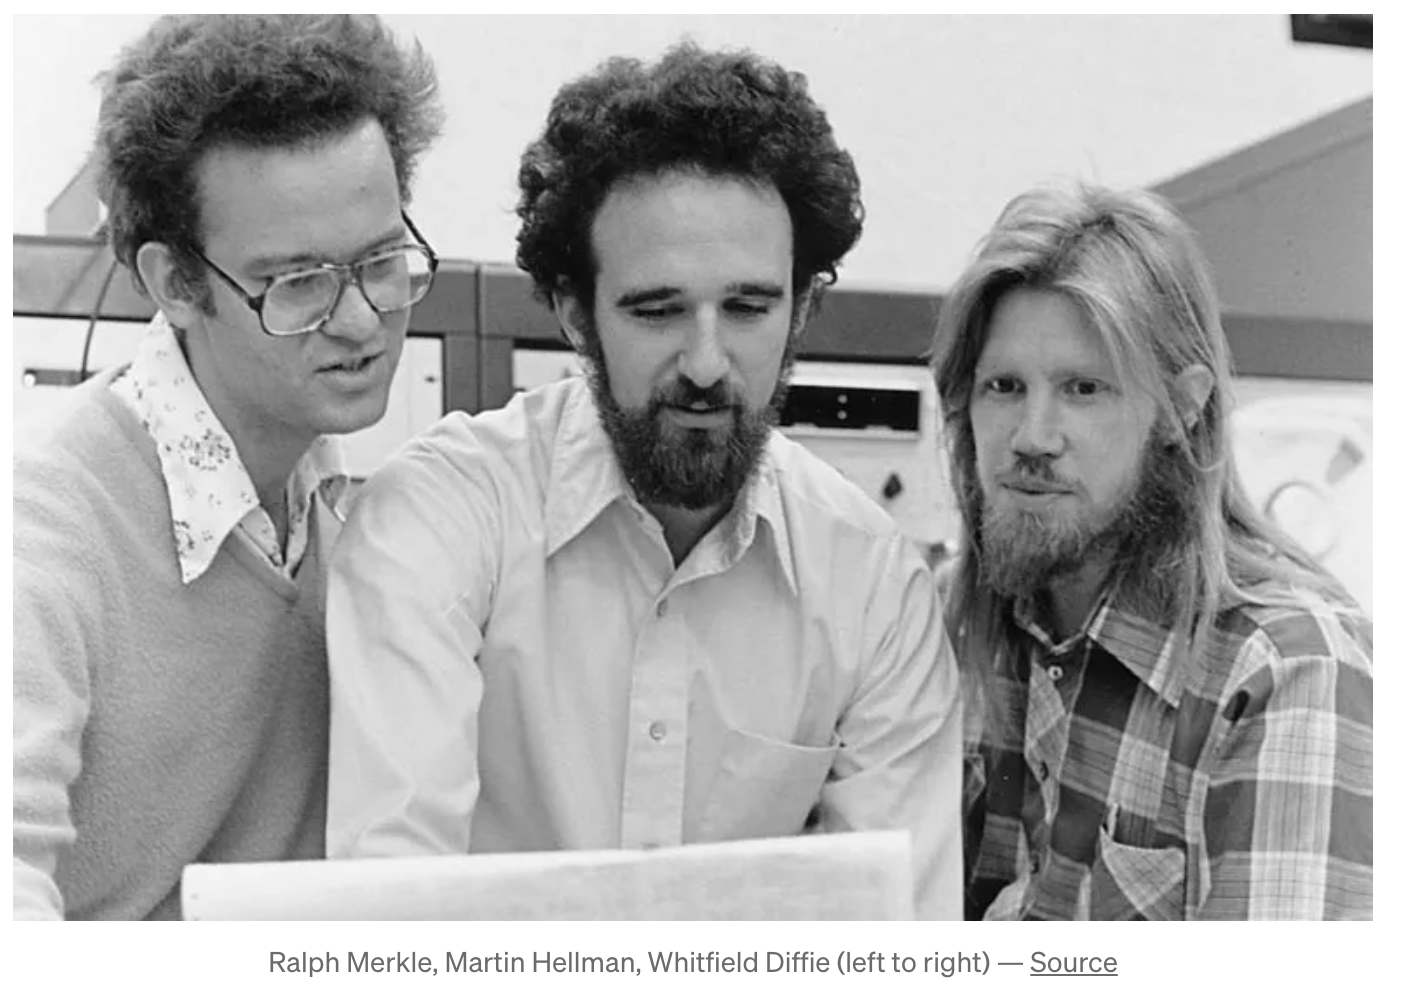
\includegraphics[width=0.8\linewidth]{Praktikum/LPU/Images/Diffie-Hellman-Merkle.png}
	\caption{ Whitfield Diffie, Martin Hellman und Robert Merkle}
	\label{fig:diffieHellmanMerkle}
\end{figure}

Wir wollen zunächst die Grundidee des Schlüsselaustauschs anhand von Farbmischungen verantschaulichen. Achten Sie auf die Farbmengen in untenstehender Abbildung \ref{fig:diffieHellmanFarbig}. 

\begin{figure}[H]
	\centering
	\begin{tikzpicture}[
		glass/.style={draw, fill=white, minimum width=1.5cm, minimum height=2cm, rounded corners=0.2cm, thick},
		liquid/.style={fill, minimum width=1.4cm, minimum height=#1, rounded corners=0.1cm},
		cup/.style={draw, fill=white, minimum width=1.5cm, minimum height=1cm, rounded corners=0.2cm, thick},
		cup_liquid/.style={fill, minimum width=1.4cm, minimum height=#1, rounded corners=0.1cm},
		arrow/.style={-Latex, thick},
		text_label/.style={font=\bfseries, align=center},
		plus_minus/.style={font=\huge},
	]

		% Define colors
		\definecolor{yellow_comm}{RGB}{255,255,0} % öffentliche Farbe
		\definecolor{orange_alice_secret}{RGB}{255,102,0} % Alice Farbe
		\definecolor{cyan_bob_secret}{RGB}{0,204,204} % Bobs Farbe
		\definecolor{mixed_alice}{RGB}{255,179,0} % Yellow + Orange (Alice's gemisch)
		\definecolor{mixed_bob}{RGB}{128,236,102} % Yellow + Cyan (Bob's gemisch)
		\definecolor{final_secret}{RGB}{170,187,68} % Mixed_Alice + Cyan or Mixed_Bob + Orange
1
		% Row 0
		\node[text_label] (alice_label) at (0, 15) {Alice};
		\node[text_label] (bob_label) at (10, 15) {Bob};

		% Row 1: Gemeinsame Farbe (Common Color)
		\node[liquid=0.4cm, yellow_comm] (alice_glass_1) at (0,14) {};
		\node[text_label, font=\Large\bfseries] (gemeinsame_farbe_text) at (5, 14) {gemeinsame Farbe};
		\node[liquid=0.4cm, yellow_comm] at (10,14) {};

		% Plus sign
		\node[plus_minus] (plus_1) at (0,13) {+};
		\node[plus_minus] (plus_2) at (10,13) {+};

		% Row 2: Geheime Farben (Secret Colors)
		\node[liquid=0.4cm, orange_alice_secret] (alice_cup_1) at (0,12) {};
		\node[text_label, font=\Large\bfseries] (geheime_farben_text_1) at (5, 12) {geheime Farben};
		\node[liquid=0.4cm, cyan_bob_secret] at (10,12) {};

		% Equals sign
		\node[plus_minus] (equals_1) at (0,11) {=};
		\node[plus_minus] (equals_2) at (10,11) {=};

		% Row 3: Alice's Mixed Color
		\node[liquid=0.8cm, mixed_alice] (alice_glass_2) at (0,10) {};
		\node[liquid=0.8cm, mixed_bob] (bob_glass_2) at (10,10) {};

		% Row 4: Alice's Received (Bob's mixed)
		\node[liquid=0.8cm, mixed_bob] (alice_glass_3) at (0,8) {};
		\node[liquid=0.8cm, mixed_alice] (bob_glass_3) at (10,8) {}; 

		% Plus sign
		\node[plus_minus] (plus_3) at (0,7) {+};
		\node[plus_minus] (plus_4) at (10,7) {+};

		% Öffentlich Übertragung (Public Transmission)
		\node[text_label, font=\Large\bfseries] (public_transfer_text) at (5,10) {öffentliche Übertragung};
		\draw[arrow] (alice_glass_2.east) -- (bob_glass_3.west);
		\draw[arrow] (bob_glass_2.west) -- (alice_glass_3.east);

		% Row 5: Alice's Secret Color
		\node[liquid=0.4cm, orange_alice_secret] (alice_cup_2) at (0,6){};
		\node[text_label, font=\Large\bfseries] (geheime_farben_text_2) at (5,6) {geheime Farben};
		\node[liquid=0.4cm, cyan_bob_secret] at (10,6) {};

		% Equals sign
		\node[plus_minus] (equals_3) at (0,5) {=};
		\node[plus_minus] (equals_4) at (10,5) {=};

		% Row 6: Alice's Final Secret
		\node[liquid=1.2cm, final_secret] (alice_final_cup) at (0,4) {};
		\node[text_label, font=\Large\bfseries] (gemeinsames_geheimnis_text) at (5,4) {gemeinsames Geheimnis};
		\node[liquid=1.2cm, final_secret] at (10,4) {};
	\end{tikzpicture}
	\caption{Dieses Schema zeigt eine Abstraktion, wie das Diffie-Hellmann-Merkle Protokoll funktioniert.}
	\label{fig:diffieHellmanFarbig}
\end{figure}

Abbildung \ref{fig:diffieHellmanFarbig} zeigt eine Abstraktion, wie das Diffie-Hellmann-Merkle Protokoll funktioniert. Zu Beginn einigen sich Alice und Bob auf eine Ausgangsfarbe. Diese ist nicht geheim. Zusäzlich wählt jeder eine eigene Farbe, welcher nur er kennt. Alice mischt die öffentliche Farbe mit ihrer geheimen Farbe und schickt sie an Bob. Ebenso mischt Bob die gemeinsame Farbe mit seiner geheimen Farbe und schickt diese an Alice. Sowohl Alice als auch Bob mischen die erhaltene Farbe wieder mit ihrer eigenen Farbe. Das Endergebnis ist bei beiden gleich und entspricht dem Schlüssel, den sie von nun an verwenden können. 

\begin{myexercise}\label{ex:kommutativEigenschaft}
	Welche Eigenschaft der Farbmischung nutzen Alice und Bob, damit beide am Ende die gleiche geheime Farbe erhalten? Wie würden wir diese Eigenschaft in der Mathematik nennen? Welche mathematischen Operationen kennen Sie, die diese Eigenschaften haben?
	\begin{myanswer}
		Alice und Bob nutzen, das Faktum, dass die Reihenfolge der Farben in der Farbmischung irrelevant ist für die Endfarbe. In der Mathematik nennen wir eine Operation \textbf{kommutativ}, wenn wir die Operanden vertauschen können. Beispiele für kommutative Operationen sind die Addition und die Multiplikation. 
	\end{myanswer}
\end{myexercise}

Damit Eve nicht in der Lage ist, die geheime Farbe zu erkennen, muss die Operation für Eve irreversibel sein. Das heisst, es muss für Eve unmöglich sein, den Prozess Rückgängig zu machen. Zum Glück dies ist im konkreten Beispiel der Fall der Fall: Mischen wir gelbe und blaue Farbe zu grün so ist es extrem schwierig, aus der grünen Farbe wieder die reinen gelben und blauen Pigmente herauszutrennen. Wäre dies nicht der Fall, so könnte Eve ganz einfach Alice und Bobs geheime Farben herausfinden und damit auch die geheime gemeinsame Farbe berechnen könnte. 

\begin{myexercise}\label{ex:irreversibelEigenschaft}
	Mischen Sie zwei Farben und versuchen Sie die Ursprungsfarben wiederherzustellen. Schaffen Sie es, wenn Sie die Farben am Computer mischen und Sie die RGB-Werte der Farben kennen?
	\begin{myanswer}
		Wenn wir zwei Farben zu gleichen Anteilen mischen, so gilt $$(R_F, G_F, B_F)=(\frac{R_1+R_2}{2}, \frac{G_1+G_2}{2}, \frac{B_1+B_2}{2}),$$ wobei $(R_F, G_F, B_F)$ das Ergebnis der Mischung und $(R_1, G_1, B_1)$ und $(R_2, G_2, B_2)$ die Ursprungsfarben sind. Wenn nur das Endergebnis bekannt ist, so können wir die Ursprungsfarben nicht wiederherstellen, sofern $(R_F,G_F,B_F)\notin \{(0, 0, 0), (255, 255, 255)\}$
	\end{myanswer}
\end{myexercise}

\begin{myexercise}\label{ex:abbildungUnsicher}
	Können wir aus Aufgabe \ref{ex:irreversibelEigenschaft} schliessen, dass das Schema, welches in Abbildung \ref{fig:diffieHellmanFarbig} dargestellt wird, von Eve nicht geknackt werden kann?
	\begin{myanswer}
		Nein, da die gemeinsame Farbe Eve bekannt ist, kann sie sehr einfach die geheimen Farben von Alice und Bob herausfinden und damit auch die Geheimfarbe. 
	\end{myanswer}
\end{myexercise}

Das eigentliche Diffie-Hellman-Merkle Protokoll verwendet keien Farben, aber weisst die oben besprochenen Eigenschaften auf.

\begin{myprocedure}[Protokoll DIFFIE-HELLMAN-MERKLE (DHM)]{myprocedure:Diffie}
	\begin{description}
		\item[Ausgangssituation:] Alice und Bob haben sich zuvor öffentlich auf eine grosse Primzahl $p$ und eine positive natürliche Zahl $g$ geeinigt. Dabei ist $g$ kleiner als $p$.
		\item[Ziel:] Alice und Bob möchten gemeinsam mit einer öffentlichen Kommunikation einen Schlüssel $s_{AB}$ vereinbaren. Diesen Schlüssel darf keine Drittperson in Erfahrung bringen.
	\end{description}
	\begin{enumerate}
		\item Alice wählt zufällig eine positive ganze Zahl $a$ mit $a<p$ und hält diese geheim. Dann berechnet sie mit dieser geheimen Zahl:
		      \begin{align*}
			      x := g^a\mod p
		      \end{align*}
		      und sendet $x$ an Bob.
		\item Bob wählt zufällig eine positive ganze Zahl $b$ mit $b<p$ und hält diese geheim. Dann berechnet er die Zahl
		      \begin{align*}
			      y := g^b\mod p
		      \end{align*}
		      und sendet $y$ an Alice.
		\item Alice erhält $y$ von Bob und berechnet mit ihrer geheimen Zahl $a$ die Zahl
		      \begin{align*}
			      s_{AB} := y^a\mod p.
		      \end{align*}
		\item Bob berechnet mit dem erhaltenen $x$ und seiner geheimen Zahl $b$ die Zahl
		      \begin{align*}
			      s_{BA} := x^b\mod p.
		      \end{align*}
	\end{enumerate}
	Mithilfe der Rechengesetze der Modulo-Operation kann bewiesen werden, dass tatsächlich
	\begin{align*}
		s_{AB} = s_{BA}
	\end{align*}
	gilt und somit Alice und Bob dieselbe Zahl berechnet haben. Diese Zahl $s_{AB}$ ist der gemeinsame Schlüssel.
\end{myprocedure}

\begin{myexercise}\label{ex:selberDHM}
	Führen Sie das DHM Verfahren selber mit Ihrer/Ihrem Sitznachbarn/in aus. Verwenden Sie
	\begin{align*}
		p := 19 \quad \text{und}\quad g := 8
	\end{align*}
	(Sie können auch eigene Werte wählen) als öffentlich bekannte Schlüssel.

	\begin{myanswer}
		Sei $a=4$ und $b=7$ $$\Rightarrow x=11,\ y=8,\ S_{AB}=S_{BA}=11$$
	\end{myanswer}
\end{myexercise}

\begin{myexercise}\label{ex:DHMKnacken}
	Versuchen Sie das Kommunikationsprotokoll DHM zu knacken, indem Sie
	für die gegebenen Werte $p, g, x$ und $y$ jeweils die geheimen Zahlen $a$ und $b$ berechnen und daraus
	dann den vereinbarten Schlüssel $s_{AB}$.
	\begin{aenum}
		\item $g = 4, p = 13, x = 12, y = 3$
		\item $g = 5, p = 7, x = 6, y = 2$
	\end{aenum}
	\begin{myanswer}
		\begin{aenum}
			\item $a = 3, b = 2$ und $s_{AB} = 12^{2}\mod 13 = 1 = 3^4 \mod 13 = S_{BA}$
			\item $a = 3, b = 4$ und $s_{AB} = 6^4\mod 7 = 1 = 2^3 \mod 7 = S_{BA}$
		\end{aenum}
	\end{myanswer}
\end{myexercise}

Die Funktion $r=g^x \mod p$ wird diskrete Exponentialfunktion genannt und ist auch für grosse Exponenten (auch mit mehr als 100-Bit) für den Computer in unter einer Sekunde berechenbar. Die Inversefunktion (Berechnung von $x$ bei gegebenem $r, g, \text{und} p$) heisst diskreter Logarithmus. Die diskrete Logarithmus Funktion ist bis heute höchst aufwändig zu berechnen. 

\begin{mychallenge}\label{ex:DHMBeweis}
	Beweisen Sie, dass $$S_{AB} = S_{BA}.$$ 

	\begin{myanswer}
		Wir zeigen, dass \begin{align*} g^{a\cdot b}\mod p = (g^a\mod p)^b\mod p.\end{align*}
		Aus der Defintion von \begin{align*}x=g^a \mod p\end{align*} folgt 
			\begin{align*} \exists m\in \Z : mp + x = g^a.\end{align*}
		Somit ist 
			\begin{align*}g^{ab}=(mp+x)^b \overset{(1)}{=}\sum_{k=0}^b {b\choose k} (mp)^kx^{b-k}.\end{align*} 
		(1) Hier haben binomischen Lehrsatz angewendet. \\
		Der einzige Summand, der kein Vielfaches von $p$ ist, ist $x^b$.
		\begin{align*}
			g^{a\cdot b} \mod p &=(mp+x)^b\mod p \\ &= \left(\sum_{k=0}^b {b\choose k} (mp)^kx^{b-k}  \right)\mod p \\ &= x^b \mod p \\ &= (g^a \mod p)^b \mod p
		\end{align*}

		Daher folgt
		\begin{align*}
			S_{AB}&=(g^a\mod p)^b\mod p = g^{a\cdot b}\mod p \\&= g^{b\cdot a}\mod p = (g^b \mod p)^a\mod p = S_BA.
		\end{align*}\qed
	\end{myanswer}
\end{mychallenge}

\section{Lernziele Diffie-Hellman-Merkle}

\begin{todolist}
  \item Ich weiss, was das Schlüsselaustauschproblem ist.
  \item Ich weiss, wie das Diffie-Hellman-Merkle Protokoll einen Schlüsselaustausch implementiert. 
  \item Ich kann für gegebene $g, p, a, \text{und } p$ den geheimen Schlüssel mittels des Diffie-Hellman-Merkle Protokolls berechnen.
  \item Ich kann erklären, warum Kommutativität für das Diffie-Hellman-Merkle Protokoll wichtig ist.
\end{todolist}

